\documentclass[12pt, a4paper, simple]{eskdtext}

\usepackage{hyperref}
\usepackage{_env/gpi_global.env}
\usepackage{_env/gpi_report.env}
\usepackage{_sty/gpi_lst}
\usepackage{_sty/gpi_toc}
\usepackage{_sty/gpi_t}
\usepackage{_sty/gpi_p}
\usepackage{_sty/gpi_u}

% Код
% \ESKDletter{О}{Л}{Р}
% \def \gpiDocTypeNum {81}
% \def \gpiDocVer {00}
% \def \gpiCode {\ESKDtheLetterI\ESKDtheLetterII\ESKDtheLetterIII.\gpiStudentGroupName\gpiStudentGroupNum.\gpiStudentCard-0\gpiDocNum~\gpiDocTypeNum~\gpiDocVer}

\def \gpiDocTopic {Отчёт лабораторной работы №\gpiDocNum}

% Графа 1 (наименование изделия/документа)
% \ESKDcolumnI {\ESKDfontII \gpiTopic \\ \gpiDocTopic}

% Графа 2 (обозначение документа)
% \ESKDsignature {\gpiCode}

% Графа 9 (наименование или различительный индекс предприятия) задает команда
% \ESKDcolumnIX {\gpiDepartment}

% Графа 11 (фамилии лиц, подписывающих документ) задают команды
% \ESKDcolumnXIfI {\gpiStudentSurname}
% \ESKDcolumnXIfII {\gpiTeacherSurname}
% \ESKDcolumnXIfV {\gpiTeacherSurname}

\begin{document}
    \begin{ESKDtitlePage}
    \ESKDstyle{empty}
    \begin{center}
        \gpiMinEdu \\
        \gpiEdu \\
        \gpiKaf \\
    \end{center}

    \vfill

    \begin{center}
        \gpiTopic
    \end{center}

    \vfill

    \begin{center}
        \textbf{\gpiDocTopic} \\
        ПО ДИСЦИПЛИНЕ \gpiDiscipline \\
    \end{center}

    \vfill

    \begin{flushright}
        \begin{minipage}[t]{7cm}
            Выполнил:\\
            \PageTitleStudentInfo
            \PageTitleDateField
            \hspace{0pt}

            Проверил:\\
            \PageTitleTeacherInfo
            \PageTitleDateField
        \end{minipage}
    \end{flushright}

    \vfill

    \begin{center}
        \PageTitleCity~\ESKDtheYear
    \end{center}
\end{ESKDtitlePage}

    \ESKDstyle{empty}
    \begin{center}
        \textbf{\gpiDocTopic}
    \end{center}

    % = = = = = = = =
    \paragraph{} \textbf{Тема}: <<\gpiTopicRep>>

    \paragraph{} \textbf{Цель}:
    приобрести практические навыки разработки многооконных приложений на JavaFX для работы с базами данных.

    \paragraph{} \textbf{Что нужно сделать}:
    долго писать.
    Реализуй табличку с CRUD операциями.

    \paragraph{} \textbf{Разработка дизайна}:

    \begin{figure}[!h]
        \centering
        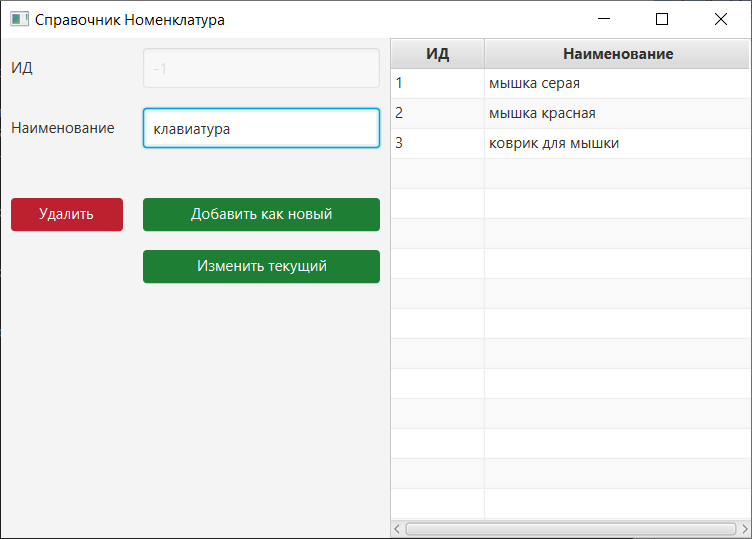
\includegraphics[]
            {_assets/RM_Nomenclature.png}
        \caption{Справочник Номенклатура}
    \end{figure}

    \paragraph{} \textbf{Исходный код}: 

    \lstinputlisting[language=java, name=src/main/java/com/example/.../Main.java]
    {../sources/src/main/java/com/example/spp_2sem_po4_galanin_lab4/Main.java}

    \lstinputlisting[language=java, name=src/main/java/com/example/.../Database.java]
    {../sources/src/main/java/com/example/spp_2sem_po4_galanin_lab4/Database.java}

    \lstinputlisting[language=xml, name=src/main/resources/com/example/.../main-window-view.fxml]
    {../sources/src/main/resources/com/example/spp_2sem_po4_galanin_lab4/main-window-view.fxml}

    \lstinputlisting[language=java, name=src/main/java/com/example/.../MainWindow.java]
    {../sources/src/main/java/com/example/spp_2sem_po4_galanin_lab4/MainWindow.java}

    \lstinputlisting[language=java, name=src/main/java/com/example/.../MainWindowController.java]
    {../sources/src/main/java/com/example/spp_2sem_po4_galanin_lab4/MainWindowController.java}

    \lstinputlisting[language=xml, name=src/main/resources/com/example/...\\/reference-book-nomenclature-window-view.fxml]
    {../sources/src/main/resources/com/example/spp_2sem_po4_galanin_lab4/reference-book-nomenclature-window-view.fxml}

    \lstinputlisting[language=java, name=src/main/java/com/example/.../ReferenceBookNomenclatureModel.java]
    {../sources/src/main/java/com/example/spp_2sem_po4_galanin_lab4/ReferenceBookNomenclatureModel.java}

    \lstinputlisting[language=java, name=src/main/java/com/example/...\\/ReferenceBookNomenclatureWindowController.java]
    {../sources/src/main/java/com/example/spp_2sem_po4_galanin_lab4/ReferenceBookNomenclatureWindowController.java}

%     \begin{lstlisting}[caption=Вывод в консоль]
%  Hello, World!
% \end{lstlisting}

    \paragraph{} \textbf{Вывод}:
    Реализовали операции CRUD: create, read, update, delete.

    Создали TableView, который выводит содержание таблицы.

    Создали форму, которая по нажатию кнопки "Добавить как новый",
    создаст новый кортедж в таблице.

    При выборе поля из TableView, данные переносятся в форму, а при замене полей и нажатии кнопки "Изменить текущий",
    добавляется в базу данных обновленный кортедж.

    При выборе поля из TableView, данные переносятся в форму, а при нажатии кнопки "Удалить",
    удаляется кортедж из базы данных. 

    % = = = = = = = =
    % \newpage
    % \addcontentsline{toc}{section}{Список использованных источников}
    % \section*{Список использованных источников}
    \paragraph{} \textbf{Список использованных источников}:
    \begin{enumerate}
        \item[1.] IntelliJ database connection error: java.sql.SQLException: No suitable driver found. SOLVED - YouTube [Электронный ресурс]
        - Режим доступа: \url{https://www.youtube.com/watch?v=lks1NZCnvL8}.
        Дата~доступа:~02.05.2022.
        \item[2.] Releases · xerial/sqlite-jdbc [Электронный ресурс]
        - Режим доступа: \url{https://github.com/xerial/sqlite-jdbc/releases}.
        Дата~доступа:~02.05.2022.
        \item[3.] JDBC CRUD Example Tutorial [Электронный ресурс]
        - Режим доступа: \url{https://www.javaguides.net/2018/10/jdbc-crud-example-tutorial.html}.
        Дата~доступа:~03.05.2022.
        \item[4.] java - Проверить наличие таблицы в БД и если она не существует создать. JDBC - Stack Overflow на русском [Электронный ресурс]
        - Режим доступа: \url{https://ru.stackoverflow.com/questions/623653/%D0%9F%D1%80%D0%BE%D0%B2%D0%B5%D1%80%D0%B8%D1%82%D1%8C-%D0%BD%D0%B0%D0%BB%D0%B8%D1%87%D0%B8%D0%B5-%D1%82%D0%B0%D0%B1%D0%BB%D0%B8%D1%86%D1%8B-%D0%B2-%D0%91%D0%94-%D0%B8-%D0%B5%D1%81%D0%BB%D0%B8-%D0%BE%D0%BD%D0%B0-%D0%BD%D0%B5-%D1%81%D1%83%D1%89%D0%B5%D1%81%D1%82%D0%B2%D1%83%D0%B5%D1%82-%D1%81%D0%BE%D0%B7%D0%B4%D0%B0%D1%82%D1%8C-jdbc}.
        Дата~доступа:~03.05.2022.
        \item[5.] SQL INSERT INTO Statement [Электронный ресурс]
        - Режим доступа: \url{https://www.w3schools.com/sql/sql_insert.asp}.
        Дата~доступа:~03.05.2022.
        \item[6.] SQL SELECT Statement [Электронный ресурс]
        - Режим доступа: \url{https://www.w3schools.com/sql/sql_select.asp}.
        Дата~доступа:~03.05.2022.
        \item[7.] SQL UPDATE Statement [Электронный ресурс]
        - Режим доступа: \url{https://www.w3schools.com/sql/sql_update.asp}.
        Дата~доступа:~03.05.2022.
        \item[8.] SQL DELETE Statement [Электронный ресурс]
        - Режим доступа: \url{https://www.w3schools.com/sql/sql_delete.asp}.
        Дата~доступа:~03.05.2022.
        \item[9.] SQL DROP TABLE Statement [Электронный ресурс]
        - Режим доступа: \url{https://www.w3schools.com/sql/sql_drop_table.asp}.
        Дата~доступа:~03.05.2022.
        \item[10.] Как создать исполняемый jar файл в IntelliJ IDEA - YouTube [Электронный ресурс]
        - Режим доступа: \url{https://www.youtube.com/watch?v=tA8rEz_xFrQ}.
        Дата~доступа:~01.05.2022.
        \item[11.] Export JavaFX 11, 15 or 17 projects into an executable jar file with IntelliJ [2022] - YouTube [Электронный ресурс]
        - Режим доступа: \url{https://www.youtube.com/watch?v=F8ahBtXkQzU}.
        Дата~доступа:~01.05.2022.
        \item[12.] JavaFX Tutorial for Beginners - CRUD Application Part 1 - YouTube [Электронный ресурс]
        - Режим доступа: \url{https://www.youtube.com/watch?v=CGWRwpeihE8}.
        Дата~доступа:~19.05.2022.
        \item[13.] JavaFX Tutorial for Beginners - CRUD Application  with JavaFX and MySQL Part 2 - YouTube [Электронный ресурс]
        - Режим доступа: \url{https://www.youtube.com/watch?v=kpnnXit2br0}.
        Дата~доступа:~20.05.2022.
        \item[14.] DemoCRUD-JavaFX/MainController.java at master · xemacscode/DemoCRUD-JavaFX [Электронный ресурс]
        - Режим доступа: \url{https://github.com/xemacscode/DemoCRUD-JavaFX/blob/master/src/org/xemacscode/demo/MainController.java}.
        Дата~доступа:~20.05.2022.
    \end{enumerate}
    \newpage
\end{document}
